%Empieza configuracion de capitulo

\setstretch{1.0}
\titleformat{\chapter}[block]{\Large\bfseries}{CHAPTER 
\Huge\thechapter\vspace{25 pt}}{0 pt}{\\\fontsize{26}{36}\selectfont}
\titlespacing{\chapter}{0 pt}{30 pt}{50 pt}[0 pt]
\titleformat{\section}{\Large\bfseries}{\thesection}{0 pt}{\hspace{30 pt}}
\titleformat{\subsection}{\large\bfseries}{\thesubsection}{0 pt}{\hspace{30 pt}}
\pagestyle{fancy}
\fancyhead[LO,LE]{\footnotesize\textit{\leftmark}}
\fancyhead[RO,RE]{\thepage}
\fancyfoot[CO,CE]{}
%Termina configuracion de capitulo

\chapter{Introduction} %Cambia Introducci'on al nombre de tu capitulo
\setstretch{1.5} %Regresa el interlineado a 1.5

\normalsize

This work presents a detailed study of how a network of embedded systems
collaborates among each others to solve parallel problems. At the end a
detailed case of study based on: industrial benchmarks for distributed systems,
power consumption analysis and optimal operating system selection, will provide
the IoT and embedded industry a solid methodology to use their compute power as
much as possible.

\section{Background}
\vspace{30 pt}
\noindent

The evolution of computing technology as made incredible progress in the
roughly 60 years since the first general-purpose electronic computer was
created. Today, less than 300 dollars  will purchase a personal computer that
has more performance, more main memory, and more disk storage than a computer
bought in 1985 for 1 million dollars. \cite{Hennessy}. This advantages has been
possible thanks to the innovations in computer design and software design.


%Computter architecture
Since the commercial use of computers (started in 1951 with the
introduction of UNIVAC \cite{Nur}) the development of the computers has had
multiple changes, not only from the architectural point of view but also from
the application point of view. In \cite{Hennessy} the image \textit"{Figure 1:1
Growth in processor performance since the mid-1980s."} shows the evolution of
the computers in term of performance over the years. 

The first important breakpoint in the history of computers came in the late
1970s, whit the emergence of the microprocessor. Since then there has been an
increase in the number of computer business being based on microprocessors. 

The 1980s saw the rise of the desktop computer based on microprocessors, in the
form of both personal computers and workstations. The 1990s saw the emergence
of the Internet and the World Wide Web, the first successful lap top computing
devices, and the emergence of high performance compute systems for business
purposes (servers). During this years the performance of the microprocessors
increase around 27\% each year.\cite{Hennessy}

However in the beginning of 2000's a dramatic change in the computer
architecture happened. The idea of increasing of computing performance in
processors, based on simply screwing up the clock frequency, could not longer
be hold. Due to the fact that the power density (amount of power per unit
volume) increase with the increase in frequency.

The solution, in order to still meet Moore's law, was the shifting to real
parallelism by doubling the number of processors on one chip die. This was the
birth of the multi-core area. This idea increasing the compute power limiting
the power density at the same time. This new computer architecture break the
paradigm of use low compute power microprocessors for embedded platforms.
Instead of this it was possible to have more compute power with less frequency.
Thanks to this radical change there has been a rapid evolution of the compute
and multimedia capabilities of embedded systems. At the point where have more
computer power in our cellphones than all of NASA back in 1969 \cite{Michio}


%Embedded architecture

But the smart-phones are not the only example of embedded platforms.
According to \cite{Hallinan} \textit{"An embedded system is a special-purpose
system in which the computer is completely encapsulated by the device it
controls"} Unlike a general-purpose computer, such as a personal
computer, an embedded system performs pre-defined tasks, usually with very
specific requirements. Examples of these are:microwaves, washing machines, printers,
and GPS (Global Positioning System) systems. All those electronic
gadgets that started to emerge 15 years ago \cite{Nur}.

The variety of the embedded applications requires at the widest spread
of processing power and cost. They include 8-bit and 16-bit processors that may
cost few cents, 32-bit microprocessors that execute 100 million instructions
per second and cost less than few dollars, and high-end processors for the
newest video games or network switches that cost at least 100 dollars and can
execute a billion instructions per second.\cite{Hennessy}

%Ubicuos systems
The combination of all these factors (the cost, size, and power density
reduction) in combination with the increase in computing power and connectivity
has caused the computing technology to evolve into ubiquitous computing.
According to Mark \cite{Mark}, ubiquitous computing is \textit{"the method of
enhancing computer use by making many computers available throughout the
physical environment, but making them effectively invisible to the user"}. This
mean that the computing power is available anywhere and at any time

%IoT

According to \cite{Nur}, currently we are moving from ubiquitous computing into
advanced ubiquitous computing. An advanced ubiquitous computing is an extension
of ubiquitous environment that improve connectivity between devices. The major
characteristics of this environment can be listed as follows: large number of
heterogeneous devices, new communication technology  and Internet of Things
(IoT) among others.


One of the most accurate definitions of the IoT is the one given by
\cite{Bahga} where it mentions that \textit{"Internet of Things refers to
physical and virtual objects that have unique identities and are connected to
the internet to facilitate intelligent applications [...] smarter"}. The IoT
enables the interconnection via the Internet of computing devices embedded in
everyday objects, enabling them to send and receive data. As you can see the
differences with traditional embedded systems are the internet connectivity and
less power consumption. IoT systems must always be connected to the internet
which require a lower power consumption.

But the entire picture of an IoT solution is quite bigger. A full solution has 
the following parts (figure~\ref{fig:1.1}).

\begin{itemize} 

\item The Thing (computing devices):  in the Internet of Things, can be a
person with a heart monitor implant, a farm animal with a bio chip transponder,
an automobile that has built-in sensors to alert the driver when tire pressure
is low or any other natural or man-made object that can be assigned
an unique identifier and provided with the ability to transfer data over a network.

\item Network Connection: Network Connections provides connectivity between
your computing devices  and the Internet, a network, or another compute device.

\item Cloud Computing Data centers for storage and Big Data analysis: The data
by itself is not useful to the end user. An alarm or recommendation is all that
the end user will matter. After the data is sent and stored into the Cloud
Computing Data Centers is necessary to run Big Data solutions that present
meaningful information to the users.

\item Presentation Devices: At the end of the day, what do we do with all that
information we have collected; one obvious thing is to display the information
via a dashboard. Dashboards have to be hosted on some kind of display, we call
that the Presentation Device.  It could be a desktop computer running an
application, a tablet or a smart phone accessing to a web page. It could even
be a purpose-built device like a retail kiosk, intelligent vending machine or a
control panel. The goal is to present the information coming from the big data
analysis.

\end{itemize}

\begin{figure}[H]
\centering
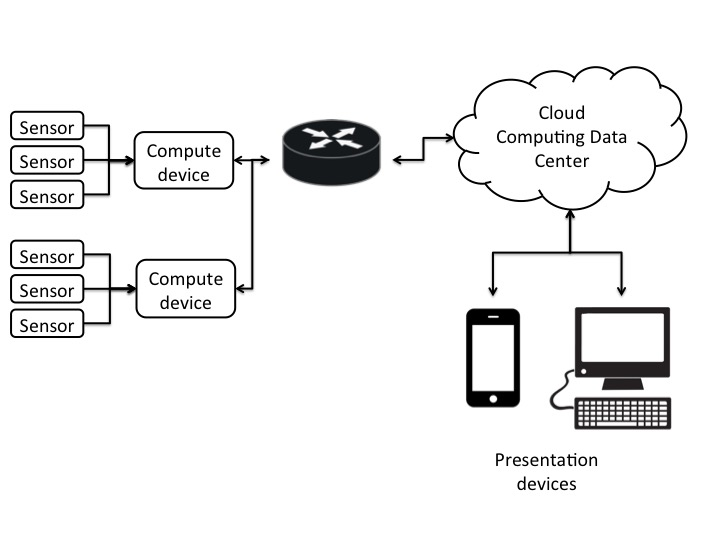
\includegraphics[width=0.75\textwidth]{images/IoT_diagram.jpg}
\caption{IoT full diagram }
\label{fig:1.1}
\end{figure}

Like many booming areas of technology, the IoT revolution is plagued by a lack
of industry standards. As you can imagine there are thousands of computing
devices and sensors from different vendors that appear on the market  every day
, each one with his unique way to send  or store their data in their
centralized cloud computing centers.

Right now exist two main projects that are compiling to establish standards for
the IoT communications: 

\begin{itemize}
\item Open Connectivity Foundation(OCF): The OCF tries to  create a set of open
specifications and protocols to enable devices from a variety of manufactures
to securely and seamlessly interact with one another. Regardless of the
manufacturer, operating system or chipset the devices that adhere to
the OCF specifications should communicate together.\cite{Terry}

\item AllSeen Alliance (AllJoyn before) : is an open source project for the
development of a universal software framework aimed at the interoperability
among heterogeneous devices, dynamic creation of proximal networks and
execution of distributed applications. The framework provides a common
interface towards smart devices \cite{Massimo}
\end{itemize}


Both standards try to solve a simple problem: communications standards among
the industry. This means that all the IoT devices could communicate among each
others despite the vendor. Despite the efforts of both initiatives none of
those are the standard in terms of IoT technology. 

In the meantime the Internet of Things revolution is here whether we like it or
not. We live in houses with computers inside our air conditions, televisions
and cars; many of them connected to the internet, but as we have seen there are
parts that are being missing. Despite the efforts to develop standard network
protocols for IoT systems there is no effort to make the IoT systems analyze
their data among each others instead of send  all the data to Cloud Data
centers to be analyzed. This could be a problem in a short future because as we
and  the solution might not to add another server (specially when you have
space and economic constrains)


\section{Problem Definition}
\noindent

The fact that use of IoT devices is rising quickly, ( according to
\cite{Benkhelifa} by 2022 is expected to have 14 billions of IoT devices ) is
creating a rise of data processed, transmitted and stored. Taking the scenario
where all these IoT devices try to send 1 kilobyte of data to the centralized
servers at the same time; this will create so much traffic that might be
similar to a security attack \footnote{ In the DDoS attack, high amount of network
traffic with maximum performance are generated and transmitted  to the
target systems\cite{Yang})}, collapsing the centralized data centers.

Apart from the problems of data transmitted, the power consumption of the
compute systems that storage and process the data generated by the IoT devices
is a key part to considerate. If current trends continue, a system to handle
the IoT data will require 100 megawatts. \cite{Xizhou}. 

Despite the variety of IoT applications, \cite{Liu-Dan} \cite{Du}, all of them are
based on the same IoT principle of send data over the internet to a centralized
processing system without using the processing capabilities of the IoT device.
In many IoT designs \cite{Du} is used a dedicated microprocessor just to transmit
data to the centralized control system; meanwhile, the intelligence in this
centralized control system is just a simple conditional rule. On the other hand
there are very few examples \cite{Wun} where the compute power of the embedded
platforms is exploited. If the IoT industry continue creating solutions without
the appropriate use of the compute power of the embedded platform and sending
all the data over the Internet; soon there will be more critical examples as
the Boeing 787 \footnote{ The Boeing 787 aircraft ordered by Virgin Atlantic
for delivery dramatically increases the volume of data the airline will need to
deal with (half terabyte in a transatlantic flight). Because they can't handle
that much terabytes of data everyday coming from various airplanes they are
looking for adding servers inside the airplanes \cite{Virgin}}

This research work tries to solve the problem of the correct use (one that take
advantage of the compute power) of all the IoT platforms in order to reduce the
amount of data transmitted as well as the amount of high performance servers
needed for data processing. 


\section{Main Objective}
\noindent

The main objective of this work is to show how an IoT networks could be self
sustainable. It means to make them solve their own compute problems without the
need to send millions of data to the cloud data centers. The work will provide
a way know when is really necessary to send the data to the cloud data centers.
It will be based on the maximum number of embedded platforms that provides the
maximum level of performance with the less amount of power consumption. At the
same time a list of applications that are good candidates for this approach is
presented. 

This work will provide the IoT industry a way  to determine if their
applications can take advantage of the communication betwen their IoT devices
to process their own data instead of sending the information to data centers.

\section{Hypothesis}
\noindent

As we have seen unsustainable power consumption have driven the microprocessor
industry to integrate multiple cores on a single die, or multicore, as an
architectural solution in order to increase the performance. The same approach
might be followed in the current IoT problem recently described. Creating a
self sustainable network of IoT systems, where the processing problems that
they have could be solved among each others with parallel computing technology
(communication among distributed clusters)

With the current compute power of the ultra-low-voltage microprocessors
platforms (core systems of the IoT devices) is possible to create a cluster
with the optimal number of embedded platforms. All of the inter-connected in a
network that provides the maximum level of performance with the less amount of
power consumption. This characteristic is determined by the power efficiency of
the network. The power efficiency is quantified by performance per watt
\cite{Jun}

The critical part is to determine the breaking point where is better to send
the data to the cloud data centers. How many systems is the maximum that these
kind of network could support and still being a good option in terms of energy
efficiency

The development of metrics to evaluate energy efficiency on the basis of
performance and power models is described in \cite{Dong}. According to
\cite{Dong} the formula for performance per watt (Perf/W), which represents the
performance achievable at the same cooling capacity, based on the average power
is as described in \ref{eq:1}:

\begin{equation}\label{eq:1}
\frac{Perf}{W} = \frac{1}{(1 + (n -1 ) k (1 - f))}
\end{equation}

Where \textit{n} is the number of processors,  \textit{f} is the fraction of
computation that programmers can parallelize  ( form 0 to 1 ) and \textit{k}, to
represent the fraction of power the processor consumes in idle state  ( from 0
to 1 )

In \cite{Dong} their analysis clearly demonstrates that a symmetric many-core
processor can easily  lose its energy efficiency as the number of cores
increases. To achieve the  best possible energy efficiency, their  work
suggests a many-core alternative, featuring many small, energy-efficient cores
integrated with a full-blown processor. They also show that by knowing the
amount of parallelism available in an application prior to execution, is
possible to  find the optimal number of active cores for maximizing performance
for a given cooling capacity and energy in a system

Is because of this that we have the hypothesis that the energy efficiency in a
cluster of ultra-ultra low power platforms will have a similar behavior that
the one presented in \cite{Dong} , with the difference that \textit{n} will be
the number of ultra-low power platforms instead of cores. 

A simulation to illustrate the hypothesis is described in figure~\ref{fig:1.2}.
In the beginning the increment of the number of nodes in our network will
increment the performance (the top part of the equation), but at the same time
the amount of watts will increase making the energy efficiency flat at some
point (if the lower part of the equation increases the equation tends to
decrease)

\begin{figure}[H]
\centering
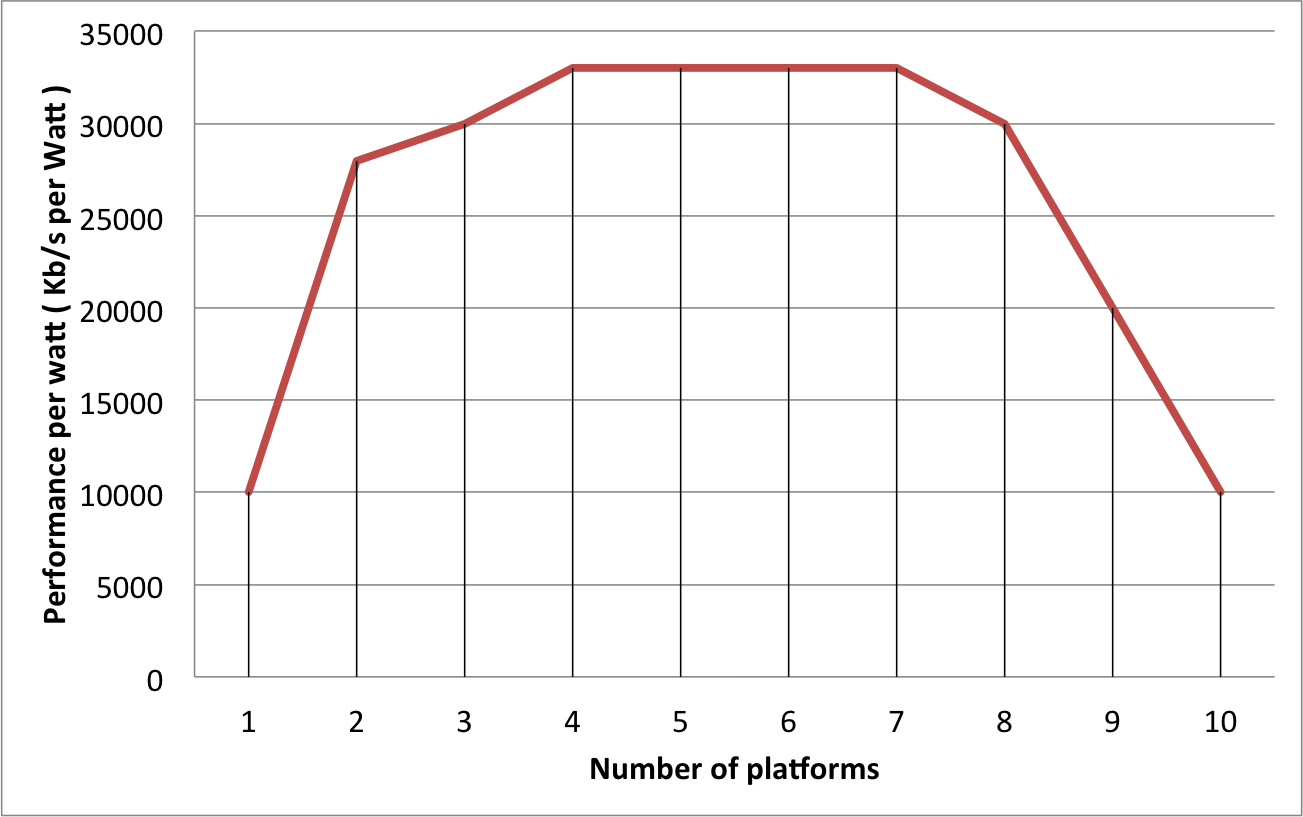
\includegraphics[width=0.75\textwidth]{images/hypothesys.png}
\caption{Hypothesis of energy efficiency behavior in embedded cluster}
\label{fig:1.2}
\end{figure}

After finding these curves for command benchmarks it will be easy for the
industry of IoT systems to determine if their applications can take advantage
of communicate their IoT devices among each others instead of sending the
information to their data centers.


\section{Methodology}
\noindent

Recent researches \cite{Saldana} \cite{Abgaria} \cite{McMahon} \cite{Liu} are 
showing an increasing interest in the topic.  All these research as always talk
about the lack of three parts: 

\begin{itemize}
\item A low-voltage microprocessors platform with enough compute power.
\item An operating system for Distributed Systems.
\item A light communication protocol to distribute the workload among the
embedded platforms.
\end{itemize}

The way we are going to address this will be:


\begin{itemize}

\item Choose the right embedded platform: There are dozens of embedded and IoT
platforms, this is why is necessary to make a deep analysis and choose the best
platform that feed our needs. (taking into consideration that sometimes the
systems might have heterogeneous platforms)

\item Choose the right communication and compute protocol: There are different
kinds of distributed compute protocols. Part of this investigation is to detect
the most reliable and suitable for our needs.

\item Choose the right performance benchmark. There are different kind of
benchmark in the cluster technology. Is necessary to find the benchmark that
cover the majority of the possible IoT applications.

\item Choose the right Operating System for the system. Once we have selected
the appropriate embedded platforms, another variable in this investigation is
the number of Operating Systems. Either if it is a micro kernel or a monolithic
kernel architecture there are more than a dozen of solutions to use.

\item Create embedded clusters to measure energy efficiency. Once we have found
the best configuration (Hardware + Operating System + Communication Protocol )
in terms of energy efficiency , we can start to create a cluster of embedded
systems.

\item Find the optimal number of embedded systems in the cluster that provide
the highest power efficiency. 

\item Release all the improvements and disagreements found as Open Source. All
the improvements made into any technology (operating systems or communication
protocols) will be published with an open source license.

\item Implement solution on real application ( greenhouse ). In order to test
the hypothesis in a real application we will implement it on a real greenhouse.
Proving that the solution give an embedded system the power of reliability and
availability without the need of external and expensive servers.
\end{itemize}

\clearpage
